\chapter{\centeering ПРОЕКТИРОВАНИЕ \\ \centeering БОЕВОЙ ЧАСТИ}
\label{cha:appendix_bch}
\emph{Кумулятивная боевая часть}

Исходные данные:
\begin{itemize}
	\item Бронепробитие по нормали 				L = 800 мм,
	\item Плотность ВВ:							$\rho_\text{вв} = 1850$ кг/$\text{м}^3$
	\item Плотность материала облицовки (медь):			$\rho_\text{об}$ = 8900 кг/$\text{м}^3$
	\item Плотность материала корпуса (алюминий):		$\rho_\text{к}$ = 2700 кг/$\text{м}^3$
\end{itemize}

Анализируя боевые части существующих ракет с подобным бронепробитием, выбираем k = 6,7. Поэтому 
$$ D=\frac{L}{k}=\frac{800}{6,7}=117,74 \text{ мм}$$

округляем до D = 120 мм

Длина БЧ:		$$ h=1,6 \cdot D=1,6 \cdot 120=192 \text{ мм}$$

Cхематично БЧ представлена на рисунке \ref{fig:appendix_bch}.
\begin{figure}
	\begin{center}
		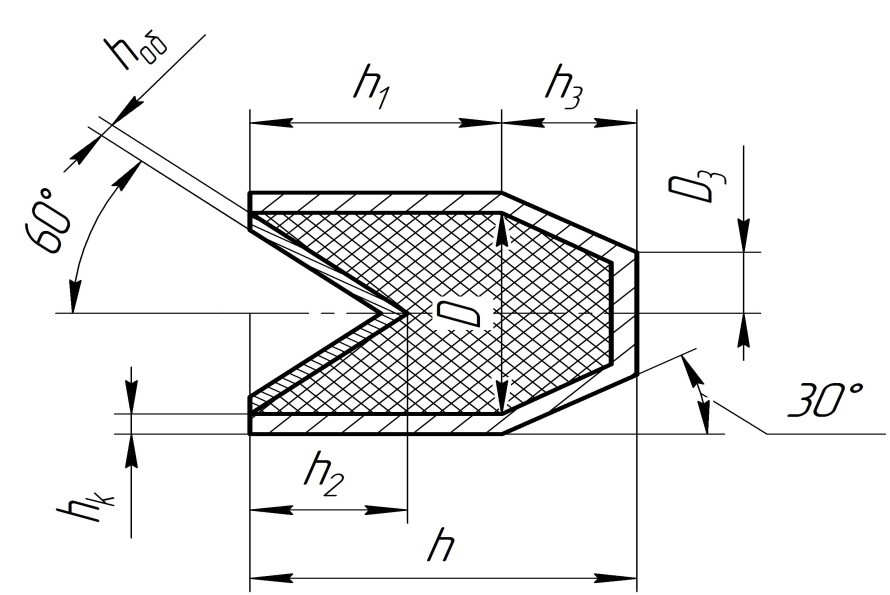
\includegraphics[height=85mm]{appendix_bch}
		\caption{}
		\label{fig:appendix_bch}
	\end{center}
\end{figure}

\clearpage
Условно поделим БЧ на 3 части:
\begin{enumerate}
	\item Цилиндрическая часть;
	\item Внутренний конус;
	\item Внешний конус.
\end{enumerate}

Цилиндрическая часть: 
\begin{enumerate}
	\item Длина: 	$h_1=1,1 \cdot D=1,1 \cdot 125 =132$ мм;
	\item Объем: 	$V_1=\pi \cdot \frac{D^2}{4} \cdot h_1=3,14 \cdot \frac{120^2}{4} \cdot 132 = 1492128 \text{ мм}^3 $;
	\item Масса:	$m_1=V_1 \cdot \rho_\text{вв}=0,000629 \cdot 1850=2,76 кг$.
\end{enumerate}


Внутренний конус:
\begin{enumerate}
	\item Длина: 	$h_2=D/2 \cdot \frac{1}{\sin 60°}  =90/2 \cdot \frac{1}{\sin 60°}  =69.28 $мм;
	\item Объем:	$V_2=\frac{1}{3} \cdot \pi \cdot \frac{D^2}{4} \cdot h_2=\frac{1}{3} \cdot 3,14 \cdot  \frac{120^2}{4} \cdot 69.28=110214 \text{ мм}^3 $;
	\item Масса:	$m_2=V_2 \cdot \rho_\text{вв}=0,0001102 \cdot 1850=0.48 кг$.
\end{enumerate}

Внешний конус:
\begin{enumerate}
	\item Длина: 	$h_3=h-h_1=192-132=60 $мм;
	\item Малый диаметр усеченного конуса: $D_3=D \cdot \tg 30° =50.7 $мм;
	\item Объем:	$V_3=\frac{1}{3} \cdot \pi \cdot \left( \frac{D^2}{4}+\frac{D}{2}  \frac{D_2}{2}+ \frac{D_2^2}{4}\right) \cdot h_3=151351 \text{ мм}^3 $;
	\item Масса:	$m_3=V_3 \cdot \rho_\text{вв}=0,000151 \cdot 1850=0.67 $ кг.
	\item Масса ВВ: $m_\text{вв}=m_1-m_2+m_3=2.76 + 0.67 - 0.48=1.95$ кг.
\end{enumerate}

Примем толщину кумулятивной воронки равной 	$h_\text{об} = 3 $ мм.

Тогда, объем материала облицовки равен 		$V_\text{об} = 32186 \text{ мм}^3$.

Масса облицовки 	$m_\text{об}=V_\text{об} \cdot \rho_\text{об}=0,0000321 \cdot 8900=0.52 $ кг.

Толщину корпуса примем равной 	$h_\text{к} = 2 $ мм.

Условно поделим корпус БЧ на 2 части:

Цилиндрическая часть
\begin{enumerate}
 \item Объем $V_1 = 13677 \text{ мм}^3$.
 \item Масса $m_\text{1}=V_\text{1} \cdot \rho_\text{к}=24454 \cdot  10^{-9} \cdot 2700=0.066$  кг.
\end{enumerate}

\clearpage
Внешний конус
\begin{enumerate}
 \item Объем $V_2 = 46940 \text{ мм}^3$.
 \item Масса $m_2=V_2 \cdot \rho_\text{к}=81652 \cdot  10^{-9} \cdot 2700=0,22 $ кг.
 \item Масса корпуса: $m_\text{к}=m_\text{1}+m_2=0,066+0,22=0.29 $ кг.
\end{enumerate}

 В кумулятивную БЧ устанавливается детонатор массой $$m_\text{дет} = 0,20 \text{ кг}$$.

 Масса кумулятивной БЧ:
 $$m_\text{БЧ}=m_\text{ВВ}+m_\text{об}+m_\text{к}+m_\text{дет}=1.95 + 0.52 + 0.29 + 0.20=2.96 \text{ кг.}$$


